%ImplementationGeneral

\subsubsection{Introduction}
We had to build our implementation around several different desires:

\begin{itemize}
\item The code has to be expandable with additional features.
\item If there is a class model, it has to be simple because the project is not that big.
\item Constants should be easy to find and adjust.
\end{itemize}

\noi According to those points, the simulation code grew to be a mixture between classes and cascaded functions. At the top is a file defining all the global constants called  \textit{defineConstants.m}. This approach is maybe not very correct in terms of a good programming style, but it makes it very simple to adjust smaller details and to keep an overview over all the constants necessary to make the model work and to specify the field the agents walk in. It also provides an easy way to store and therefore document each run by simply saving the file containing all constants to a text file. All constants and variables are considered to be in SI-Units, if not mentioned otherwise. This means that all position specifications are given in meters, the velocity in meters per second and so on. Of course, this is only an approximation of reality, but it makes comparisons possible and easy.\\

\noi There are 3 classes implemented: \textit{simulation.m}, \textit{agent.m} and \textit{drawing.m}. A further description about these classes can be found in the table beneath or directly in the header of the class files. The rest of the code is split up into different logical functions.\\[12px]
\begin{tabular}{|l|p{7cm}|l|}
        \hline
        Class & Description & Parent \\ \hline
        simulation.m
		& This class offers all the functions for simulations. It can be executed  
		with different parameters depending on the users preferences.           
		& Matlab "handle" class \\ \hline
		agent.m    
		& This class is a container for all the agent data such as its radius, velocity and 
		position.   
		& Matlab "handle" class \\ \hline
		drawing.m
		& This class can draw a field containing agents.           
		& Matlab "handle" class \\  \hline
\end{tabular}\\[12px]

\noi The class diagram given in figure \ref{fig:classpackage} is a summary of the most important functions and properties in this project.\\

\begin{figure}[h!]
	\centering
		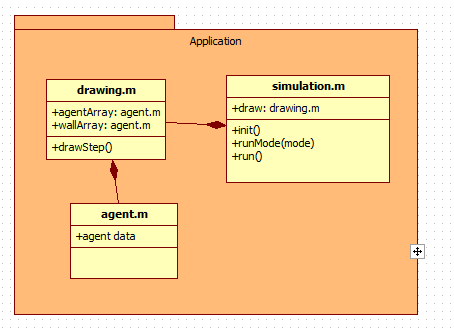
\includegraphics[width=0.70\textwidth]{pictures/classpackage}
	\caption{Class diagram of our model. From bottom to top we implemented a class \textit{agent.m}, \textit{drawing.m} and \textit{simulation.m}.}
	\label{fig:classpackage}
\end{figure}

%simulation.m
\subsubsection{Important classes to run the simulation}
\noi The simulation class \textit{simulation.m} describes an object that wraps all the different possibilities of our simulation program. It's the starting point for a new simulation, runs this simulation and collects all the data requested from the agents and the simulated environment. The drawing class \textit{drawing.m} handles all graphical aspects of our simulation. The agent class \textit{agent.m} has a subchapter of its own because it fulfills a very different role than the two classes mentioned previously.\\
The main flow of a run cycle is described in the activity diagram given in figure \ref{fig:activityDiagram}.\\


\begin{figure}[h!]
	\centering
		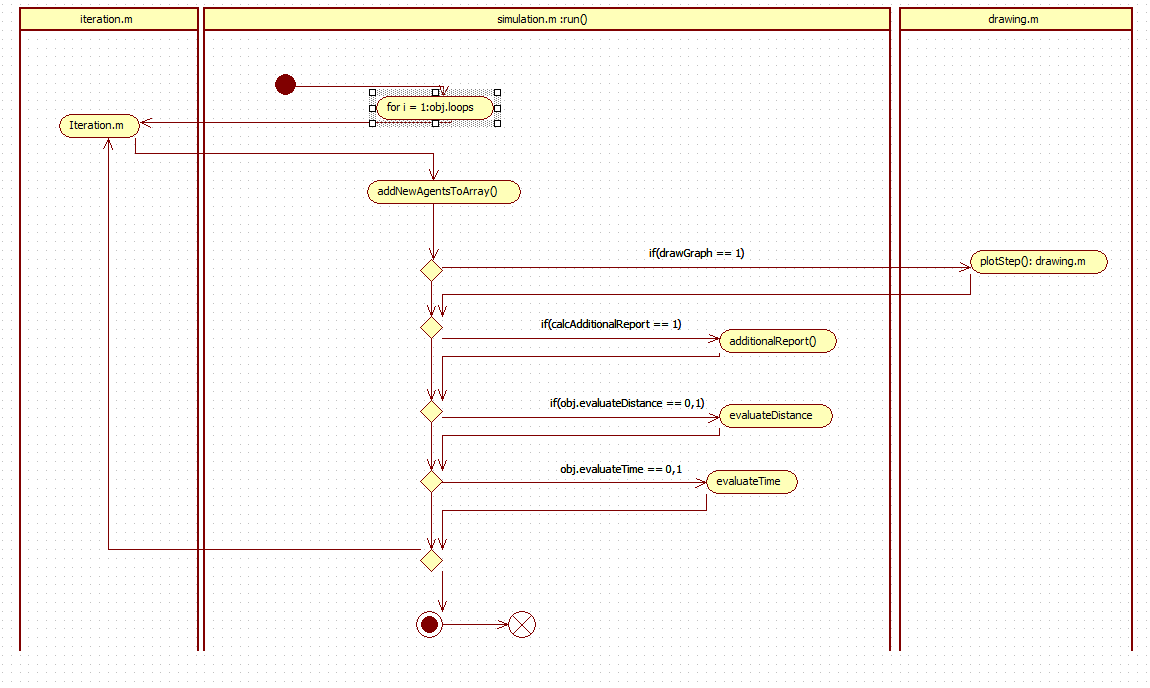
\includegraphics[width=0.70\textwidth]{pictures/activityDiagram}
	\caption{Activity diagram of our model.}
	\label{fig:activityDiagram}
\end{figure}

\noi Important properties of the simulation class \textit{simulation.m} are:
\begin{itemize}
\item \textsc{draw}: The \textit{drawing.m} implementation.
\item \textsc{result}: A matrix containing simulation results.
\item \textsc{additionalResult}: A matrix containing further simulation results.
\item \textsc{evaluateTime}: A vector used to evaluate the time an agent has spent in the simulation during its existence. %Noch beschreiben
\item \textsc{evaluateDistance}: A vector used to evaluate the distance an agent has covered in the simulation during its existence. %Noch beschreiben
\end{itemize}

\noi All methods of the simulation class are listed here:
\begin{itemize}
\item \textsc{simulation()}: Constructor, sets up the object.
\item \textsc{init()}: Initializes the existing object: Fills up arrays with empty objects, sets up vectors, etc.
\item \textsc{runMode()}: Pass console like parameters to this function to run a simulation and choose between various runmodes.
\item \textsc{additionalReport()}: Fills the additionalResult matrix with data.
\item \textsc{calcPossibleAgents()}: Calculates the maximum possible number of agents for the set area. 
\item \textsc{randPrefix()}: Randomly generates -1 or 1 to set the spawnpoint (top or bottom), if wanted to. It was replaced by spawning probabilities for top and bottom.
\item \textsc{initialSpawn()}: Fills up the agent array with new \textit{agent.m} objects. They have priority 0 which corresponds to non-existing agents.
\item \textsc{addNewAgentsToArray()}: Used to add new agents to the simulation while running.
\item \textsc{balanceProbability()}: Balances the probabilities to spawn agents, if wanted to. It was replaced by spawning probabilities for top and bottom with given constant probability.
\item \textsc{run()}: Main function to run a simulation after everything is set up and ready. This function should not be executed directly by the user. New simulations should be started with the \textsc{runMode()} function.
\end{itemize}

\noi See also the activity diagram (figure \ref{fig:activityDiagram}) for a better overview on how these method functions are used in the simulation.\\

%drawing.m
\noi The drawing class \textit{drawing.m} basically adapts simple Matlab drawing functions and converts them into useful functions for this project. As a result it's very easy to draw the new situation after a simulation step by simply calling the method \textsc{plotStep()}.

\subsubsection{Properties}
Important properties are:
\begin{itemize}
\item \textsc{particleDensity}: Resolution for wall \textit{agent.m} objects in $\frac{\y{agents}}{\y{meter}}$.
\item \textsc{width}: The field width.
\item \textsc{length}: The field length.
\item \textsc{wallArray}: All the agent.m objects for the wall.
\item \textsc{agentArray}: All the agent.m objects for the simulation.
\end{itemize}

\subsubsection{Methods}
All methods are listed here:
\begin{itemize}
\item \textsc{drawing()}: Constructor, sets up the object.
\item \textsc{createWall()}: Creates wall agents according to the settings.
\item \textsc{plotStep()}: Main function, plots all the agents on a field with the walls and the starting lines. 
\item \textsc{drawWallSquares}: Draws the walls on the side.
\item \textsc{circlePlot}: Draws circles for the agents.
\item \textsc{drawLine}: Draws a line with coordinates. Used for the direction indicators etc.
\end{itemize}
\noi How the field is created is the subject of subchapter \ref{drawField}.

\subsubsection{Simplifications}
Some simplifications and constraints on the model had to be introduced during the implementation to keep the whole simulation manageable. At first, we decided that the agents should walk either up or down and used the sign of an agent's velocity as an indication in which direction the agent goes. In the logic functions, a discretization had to be introduced for the numerical evaluations of functions. To inter-convert values between different vectors, the function \textit{closest.m} was used.\\
\noi As a consequence of the model used for the logic functions, the agents will only be able to look forwards. Because of the actual way \textit{logicFunction.m} was implemented (see subchapter \ref{logic}), they would not use the full $\pm 90^\circ$ in front and on the side of them, but almost. We thought this not to be too critical as the human visual field is also smaller than $180^\circ$, if one doesn't move the head.\\
\noi If one walks through the main station, it is visible that many people are not on their own. Groups of people tend to walk together as they want to chat. This can be seen very clearly in couples which try to walk side-by-side. To incorporate this in our model, we would have to introduce some kind of coupling between agents, for example that they would always be below a certain distance from each other. As we constructed our model from scratch, we thought it should be challenging enough to make it work with completely independent agents and decided to make every agents independent of all others.\\
\noi The hallway in the main station in Zurich is approximately 60 meters long. We shortened the way to 30 meters as we reckon that the same effects should be visible over that length. This saves some time for the simulations as the way until the agents from the opposite directions meet is considerable shortened. Also, it is of practical use as one can observe more details in a less stretched picture.

\subsection{How to run a simulation}
To start a simulation, simply change to the "/code" directory in your local matlab installation. Then type "run" into the command window. This will set up a new simulation environment. This environment can be accessed trough the "sim" variable.\\
The run script will ask for a "runmode" and whether you'd like to save the data. Supported runmodes are:\\[12px]
\begin{tabular}{|p{3cm}|p{10cm}|}
      \hline
      normal & normal mode with many wall agents\\ \hline
      fasttest & faster mode with less wall agents \\ 
      \hline
\end{tabular}\\[12px]
\noi Supported parameters are:\\[12px]
\begin{tabular}{|p{3cm}|p{10cm}|}
      \hline
      -nograph & simulation draws no graph, can be used if graphical output is not necessary.\\ \hline
      -report & additional report will be recorded\\ \hline
      -nodirections & removes the direction markers on top of the agents.\\
      \hline
\end{tabular}\\[12px]
\noi A string could be for example: "normal -nograph -report". For a more detailed example please view the header of the run.m file. \\
\noi If one wants to save the data, type "Y" when asked and type in the name of the location/filename where the data shall be stored to. As a default, they are saved into the sim folder. Then the \textit{defineConstants.m} file containing all the constants is saved as a .txt file with the runmode appended. After the simulation is finished, the workspace variables containing the "sim" variable are saved as a .mat file. The situation after the last iteration is drawn and saved as a .png file, also when the parameter -nograph was called. This allows a first visual check on how a run went.
